\chapter{Web Applikationen}

Der Gegendstand unserer Untersuchungen ist eine programmierte Webapplikation. Dieses Kapitel soll ein Grundverständnis über den Aufbau einer Webapplikation bieten.

\section{Struktur}

Eine Webapplikation besitzt sowohl eine interne Architektur (Struktur der Applikation bzw. des Source Codes) als auch eine Systemarchitektur (Integration mit externen Systemen). Eine Webapplikation wird in einer oder mehreren Programmiersprachen implementiert, zumeist unter Zuhilfenahme von Web-Frameworks bzw. -bibliotheken (diese können auch Bestandteil der Standardbibliothek einer der verwendeten Programmiersprachen sein).

Das Werk des Entwicklers ist der Source Code, welcher die benötigten Funktionen der Webapplikation implementiert. In Abhängigkeit von der verwendeten Technologie wird dieser Code auf den Applikationsserver als source code oder in kompilierter Form eingespielt und auf diesem schlußendlich auch exekutiert. Während der Exekution wird zumeist ein Applikationsserver involviert. Dieser kann entweder als eigenständiger Prozess (z. B. \textit{Apache Tomcat} als Applikationsserver für Java Servlets), innerhalb des Webservers (z. B. die Kombination von Apache Webserver mit \textit{mod\_php} für PHP) oder sogar ein Teil des kompilierten Programms sein (z. B. bei Verwendung von statischen binaries mit Go oder Rust).

Ein häufiges Problem ist die Zuordnung der Admin-Verantwortung zu den jeweiligen Komponenten. Es kann passieren, dass Entwickler davon ausgehen, dass eine Komponente von Administratoren verwaltet wird und vice versa. Dadurch kann es zum Unterlassen wichtiger Updates kommen.

\subsection{Wahl der Programmiersprache}

Zur Umsetzung einer Applikation wird eine Programmiersprache bemüht. Je nach Abstraktionslevel und Zielpublikum der Programmiersprache (bzw. des verwendeten Frameworks) ergeben sich positive und negative Auswirkungen auf die Sicherheit der Applikation.

Hierdurch sollte allerdings kein Chauvinismus bedingt werden. Es ist sowohl möglich in einer sicheren Programmiersprache unsicher zu programmieren als auch vice versa. Programmierer sollten sich der jeweiligen Eigenarten der gewählten Programmiersprache bewußt sein und ggf. vorsorglich gewisse Features nur unter Bedacht einsetzen.

Einflussreicher auf die Sicherheit der Applikation ist die Selektion von sicheren Bibliotheken und Komponenten. Hier sollten Komponenten mit einer guten Sicherheitshistorie gewählt werden, es ist essentiell, zeitnahe auch Sicherheitsupdates für verwendete Komponenten einzuspielen.

\subsection{Interne Architektur}

Die interne Struktur beschreibt, wie die Webapplikation selbst gebaut und der Code strukturiert wurde --- wie die Funtkionen auf Source-Code Komponenten aufgeteilt wurden. Die interne Architektur wird stark durch das verwendete Framework und der verwendeten Programmiersprache geprägt. Es ist sinnvoll, sich an die Annahmen und Konventionen des verwendeten Frameworks zu halten anstatt gegen diese Konventionen anzukämpfen.

\subsubsection{Request-Routing}

Ein guter Unterscheidungspunkt ist, wie der Webserver erkennen kann, dass ein eingehender HTTP Request über einen Applikationsserver, und damit als Applikationscode, ausgeführt werden soll. Initial wurde dies primär über die Dateien im Dateisystem erkannt. Gegeben ein Webroot von \url{/var/www/} und eine Datei \url{/var/www/operation.php} wird ein Aufruf der zugeordneten Webseite \url{https://www.example.local/operation.php} an die Datei \textit{operation.php} weitergeleitet und (falls PHP am server konfiguriert wurde) als PHP Applikation ausgeführt. Dieser Aufbau ist fehleranfällig: falls ein Entwickler eine .php-Datei am Server vergisst oder ein Angreifer eine zusätzliche .php-Datei am Server hochladen kann, kann es zu einer ungewollten Code-Execution kommen. Neuere Frameworks bieten zumeist die Möglichkeit, ein explizites Request-Routing zu definieren, so könnte z. B. das PHP-Framework Laraval mit folgender \url{routes/web.php} Konfiguration\footnote{\url{https://laravel.com/docs/5.7/routing}} gestartet werden:

\begin{minted}{php}
Route::get('/operation.php', 'SomeController@operation');
\end{minted}

In diesem Fall wird ein eingehender Request auf \url{/operation.php} an die Methode \textit{operation} des Controllers \textit{SomeController} weitergeleitet. Auf diese Weise wird explizit definiert, welche Operationen wie erreichbar sind und wo sich der aufzurufende Source-Code befindet.

\subsubsection{Model-View-Controller (MVC) Pattern}

Ein häufiges Muster für die interne Code-Struktur ist das MVC-Pattern. Hier wird die Funktionalität auf folgende groben Bereiche aufgeteilt:

\begin{description}
	\item[Model] ist zuständig für die Speicherung von Daten. Zumeist wird die Geschäftslogik innerhalb des Models abgebildet (\textit{thin controller, fat model}).
	\item[View]: eine View dient zur Darstellung von Daten. Zumeist wird jede einzelne Webseite über ein View-Objekt abgebildet. Mehrere View-Objekte pro Datum sind möglich, so kann z. B. das gleiche Model mittels einer View als Webseite ausgegeben ausgegeben, und mittels eines weiteren View-Objekts als Excel-Sheet heruntergeladen, werden.
	\item[Controller] akzeptiert Eingaben (z. B. HTTP- oder WebSocket-Requests), überprüft diese und interagiert mit dem Model um Geschäftsprozesse anzustossen. Um eine Antwort gegenüber dem Client zu präsentieren, werden Daten vom Controller an die View-Objekte übergeben.
\end{description}

Klassische Webapplikationen waren historisch thin-client Applikationen: die gesamte Logik wird server-seitig ausgeführt, der Client (Webbrowser) dient rein zur statischen Darstellung. Mit JavaScript entstand die Möglichkeit, innerhalb des Browsers Code auszuführen. Einige Frameworks wie \textit{Angular.js} implementieren das MVC-Pattern samt Routing innerhalb des Browsers. Der Server dient als Datenquelle und bietet jene zumeist über Webservices an.

Die Wahl der Struktur besitzt Einfluss auf Sicherheitsentscheidungen der Applikation. Bei einem klasssischen server-seitigen MVC-Pattern werden z. B. technische Überprüfungen auf Schadcode in User-Eingaben, Authentication- und Authorization-Checks innerhalb von Controllern implementiert. Wird client-seitig JavaScript verwendet, muss der server-seitige Service eine Überprüfung der JavaScript-Anfragen auf Schadcode, Authentication- und Authorization durchführen.

\subsubsection{Single-Page Applications und Progressive Web Applications}

Die Möglichkeiten von JavaScript und HTML5 wurden immer mächtiger. Dies führte zu Architekturen wie Single-Page Applications (SPA) bei denen alle Inhalte dynamisch per JavaScript geladen bzw. generiert werden.

Werden diese SPAs mit HTML5 Offline-Fähigkeiten (HTML5 localStorage) und langlebigen nebenläufigen JavaScript-Prozessen (HTML5 WebWorker) kombiniert, könnnen offline lauffähige Webseiten geschrieben werden, die klassischen Desktop-Applikationen  sehr ähnlich sind. Diese werden häufig Progressive Web Applications (PWA) genannt. Werden Daten offline gespeichert, müssen deren Integrität und Vertraulichkeit mit geeigneten Methoden gewährleistet werden.

\subsection{System-Architektur einer primitiven Web-Applikation}

Eine einfache Webapplikation wird zumeist aus drei groben Komponenten bestehen:

\begin{itemize}
	\item Webserver: dient zur Bereitstellung statischer Dateien und leitet dynamische Anfragen an die jeweiligen Applikationsserver weiter. Webserver sind optimiert für das effiziente Zustellen statischer Inhalte.
	\item Applikationsserver: beinhalten die Applikation und bieten die Laufzeitumgebung der Applikation an. Die Applikation kommuniziert mit einer Datenbank zur Speicherung dynamischer Daten.
	\item Datenbank: beinhaltet dynamische Daten.
\end{itemize}

Die Bearbeitung einer Client-Anfrage durch den Applikationsserver kann längere Zeit benötigen. Während der Bearbeitung blockiert der Applikationsserver --- um einen höheren Durchsatz und geringere Latenzzeiten zu erreichen wird häufig ein Webserver mit mehreren Applikationsservern kombiniert.

Je nach Webserver- und Applikationsserverimplementierung kann der Applikationsserver Teil des Webservers sein. Intern sind die Funktionalitäten allerdings getrennt. Im Sinne von Separation of Concerns ist es vorteilhaft, Applikationsserver und Webserver zu trennen. Dadurch ist es möglich, die unterschiedlichen Serverprozesse mit eigenständigen Benutzerrollen zu betreiben.

\subsubsection{Potentielle zusätzliche Komponenten bei Webapplikationen}

Während Webserver, Applikationsserver und Datenbank zum Betrieb einer dynamischen Webapplikation prinzipiell ausreichen, kann es zu einer Inflation von externen Komponenten kommen:

\begin{figure}[h!]
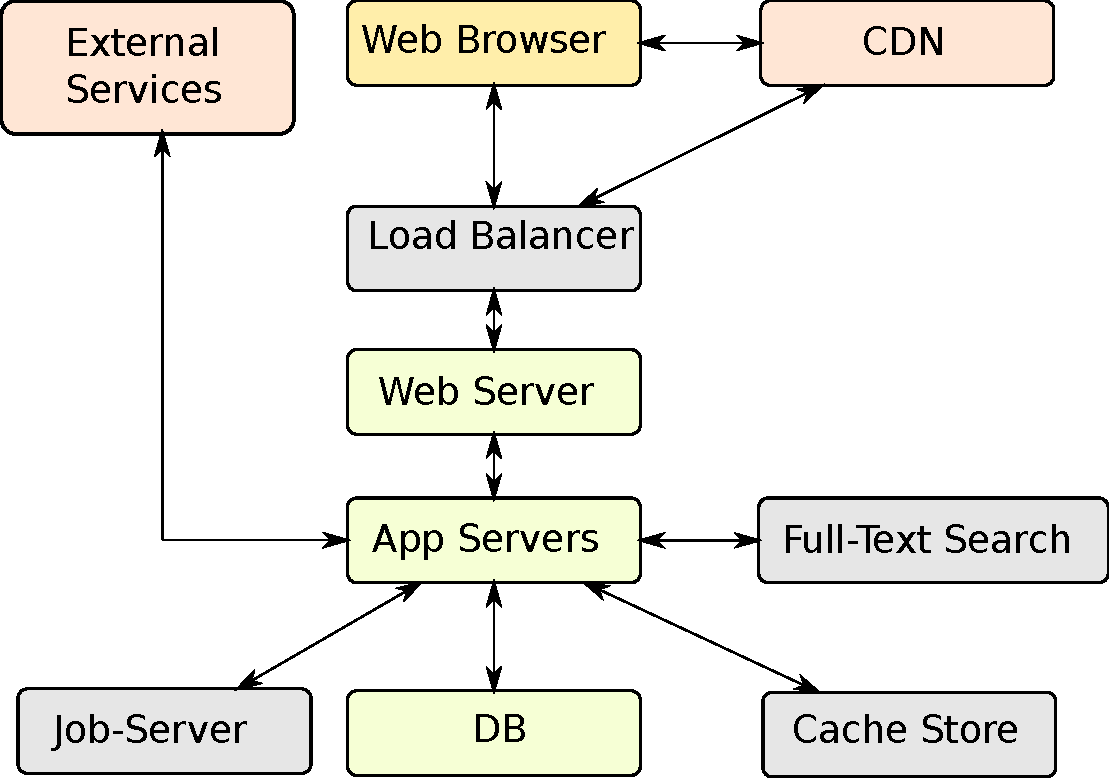
\includegraphics[width=10cm]{images/web_components.pdf}
\centering
\end{figure}

Um einige der hier vorkommenden Komponenten zu erwähnen:

\begin{itemize}
	\item Load-Balancer: verteilen den Traffic auf mehrere Webserver. Hier kann es zu Problemen beim Session-Management kommen.
	\item Content Delivery Networks (CDNs): dienen zur Performancesteigerung bei der Zustellung statischer Daten. Die Inhalte werden über ein geographisch verteiltes Netzwerk direkt an die Clients zugestellt.
	\item Caching Services werden verwendet, um häufig benötigte Daten oder Webseitenfragmente zwischenzuspeichern. Zumeist geschieht dies in-memory, bekannte Produkte sind z. B. memcached. Ein häufiges Problem ist, dass der Zugriff ohne Überprüfung der Authorisierung erfolgt. Somit erhält ein Angreifer mit Zugriff auf einen Caching Service potentiell auch Zugriff auf sensible Daten.
	\item Job Server: eine Client-Anfrage muss innerhalb kurzer Zeit beantwortet werden, falls dies nicht erfolgt kann im worst-case der Client-Browser die Verbindung unterbrechen. Um trotzdem langfristige Operationen auszuführen, können diese nebenläufig durch einen Job-Servers ausgeführt werden. Bekannte Produkte in diesem Umfeld sind RabbitMQ oder Redis. Ein potentielles Problem ist, dass Jobs Datenbankzugriffe benötigen und daher der Job Worker eine bestehende Verbindung zur Datenbank besitzt (welche von einem Angreifer ausgenutzt werden kann).
	\item Full-Text Search: viele Webapplikationen benötigen eine Volltextsuche, diese wird teilweise über einen externen Suchserver implementiert. Dieser beinhaltet eine bearbeite Version des Datenbestands der Datenbank. Ein mögliches Problem sind fehlende Berechtigungsüberprüfungen --- während auf der Datenbank der Datenzugriff zwar eingeschränkt wird, wird dies häufig innerhalb der Suchdatenbank vergessen.
	\item External Services werden häufig von Webapplikationen aufgerufen bzw. integriert. Ein Problem dabei ist, dass Webapplikationen häufig davon ausgehen, dass externe Services sich an definierte Protokolle halten.
\end{itemize}

\section{Angriffsfläche/Attack Surface}

Die Angriffsfläche ist jener Bereich, auf den ein potentieller Angreifer Zugriff erhält. Die extern sichtbare Webapplikation ist Teil der Angriffsfläche. Im Sinne der Systemsicherheit sollten Entwickler versuchen, die Angriffsfläche zu minimieren. Problematisch ist, dass die Angriffsfläche nicht nur die direkte Applikation, sondern auch alle verbundenen Funktionen und Komponenten, beinhaltet. Bei der Definition der Angriffsfläche sollten u.a. folgende Fragen gestellt werden: 

\begin{itemize}
	\item Sind interne Anwender potentielle Angreifer? In diesem Fall wären auch interne Schnittstellen Teil der Angriffsfläche.
	\item Sind Administratoren potentielle Angreifer? In diesem Fall wären auch etwaige Administrationswebseiten Teil der Angriffsfläche.
	\item Besitzt der Angreifer Zugriff auf Backups oder Logdateien?
	\item Besitzt ein Angreifer Zugriff auf externe Services und sind daher die Callbacks innerhalb der Applikation Teil der Angriffsfläche?
\end{itemize}

\subsection{Wartungszuständigkeiten}

Ein Problem bei Webapplikationen mit vielen Komponenten ist die Wartungsverantwortlichkeit. Die Applikation wird durch Softwareentwickler bereitgestellt, die Wartung der jeweiligen Komponenten erfolgt meistens durch Administratoren.

Beispiel: eine Applikation benötigt einen Java-Applikationsserver (z.B. Tomcat). Die Administratoren setzen einen Linux Server auf und installieren manuell Tomcat (Download von der Hersteller-Website) da eine spezielle Tomcat Version benötigt wird. Die Entwickler übergeben den kompilierten Source Code als war-File welches von den Admins eingespielt wird. Das Betriebssystem wird regelmäßig über dessen Update-Mechanismus upgedatet. Der Applikationsserver kann nicht automatisch upgedatet werden, da hier erst von den Entwicklern das okay kommen muss. Wer übernimmt das Update das Applikationsservers (das nicht automatisiert werden kann)?

Durch das Outsourcing von Funktionalität in die Cloud wurde dieses Problem noch verschärft, folgende Grundregeln können angenommen werden:

\begin{itemize}
	\item Self-hosted Server mit eigener Applikation: hier ist der Betreiber/Entwickler für die Wartung aller Komponenten (inkl. Firmware, Lights-out-Management/BMC, Netzwerkinfrastruktur) zuständig.
	\item Infrastructure-as-a-Service (IaaS): hier ist der Anbieter (z. B. Amazon mit seinem EC2 Dienst) für die Hardware, Virtualisierung, Firmware und Netzwerkhardware zuständig. Der eingemietete User ist für Betriebssystem, Laufzeitumgebung, lokale betriebene Hintergrunddienste wie z. B. Datenbanken und die Applikation zuständig.
	\item Plattform-as-a-Service: hier ist der Anbieter (z. B. Heroku) zusätzlich (zu den IaaS Dingen) noch für das Betriebssystem, die Laufzeitumgebung und Hintergrundservices zuständig.
	\item Software-as-a-Service (SaaS): hier ist der Anbieter der Software (z. B. gmail) für die Wartung aller Komponente zuständig.
\end{itemize}

\section{Speicherung von Passwörtern}
\label{password_storage}

Werden Passwörter durch die Applikation verarbeitet bzw. gespeichert müssen diese besonders geschützt werden. Der Grundsatz ist, dass Passwörter niemals plaintext gespeichert werden dürfen. Dies inkludiert alle Logdateien, Debug-Logs, etc. Die meisten Frameworks besitzen Möglichkeiten sensitive Felder (wie Passwortfelder) explizit vom Logging auszunehmen.

\subsection{Sichere Speicherung von Passwörtern}

Wenn Credentials unbedingt innerhalb der Applikation gespeichert werden müssen, sind Schutzmaßnahmen für deren Vertraulichkeit unabdingbar. Sie dürfen niemals in plain-text (unverschlüsselt) persistiert werden, sondern sollten so früh wie möglich mittels einer Einwegfunktion transformiert werden. Dies sollte innerhalb der Applikation und nicht erst z. B. in einer nachgelagerten Datenbank geschehen. Würde dies z. B. mittels eines Datenbanktriggers durchgeführt werden, muss die Applikation das Passwort an die DB übergeben: falls die DB nun das Passwort unsicher bearbeitet oder speichert (DB-Logs, Journal, Fehlerlogs) kann dies durch die Applikation nicht beeinflusst werden.

Als Einwegfunktion wird zumeist eine kryptographische Hash-Variante verwendet. Da Hashes auf deren Geschwindigkeit hin optimiert wurden, sind diese eigentlich suboptimal für Passwort-Hashing geeignet: durch diese Optimierung kann ein Angreifer ebenso effizient einen Brute-Force-Angriff durchführen. Aus diesem Grund sind Key-Derivation-Functions (KDFs) vorzuziehen. Dies sind Verfahren, die ``konfigurierbar langsam'' sind. Sie werden so langsam konfiguriert, dass sie im Normalbetrieb noch keinen übertriebenen negativen Impact auf die Performance besitzen, aber gleichzeitig wirkungsvoll Brute-Force-Angriffe unterbinden. Beispiele für KDFs sind \textit{PDKDF2}, \textit{bcrypt} und \textit{scrypt}.

Werden Hashes extrahiert können offline Brute-Force Angriffe gegen diese Hashes verwendet werden. Diese verwenden meistens multiple Grafikkarten und benötigen keine online Verbindung zu der Online-Applikation. Die dabei erreichten Geschwindigkeiten sind um eine Vielzahl höher als die bei Online-Brute Force Angriffen erreichte Geschwindigkeit.

\subsection{Umgang mit Credentials in Frameworks}

Innerhalb von Anwendungen müssen häufig Zugangsdaten für Fremdsysteme verwaltet werden, beispielsweise verwenden die meisten Applikationsserver im Hintergrund einen Datenbankserver oder einen Mailserver. Die Zugangsdaten für diese Server müssen in der Applikation hinterlegt werden. Geschieht dies direkt im Source Code erlangt jeder Angreifer mit dem Zugriff auf den Source Code Zugriff auf diese Zugangsdaten. Häufig geschieht es, dass solche Source Code Repositories auf privaten Versionierungsservern (VCS, Version Control Systems, wie z. B. Subversion oder Git) gespeichert, und durch eine (kurzfristige) Fehlkonfiguration diese Daten öffentlich verfügbar gemacht werden. Aus diesem Grund sollten niemals Credentials unverschlüsselt in Source Code Repositories gespeichert werden.

Als Beispiel wird hier kurz das Credential-Konzept von Ruby on Rails (Version 5.2) vorgestellt. Innerhalb des Repositories gibt es eine Datei \textit{credentials.yml.enc} in welcher Credentials bzw. private Schlüssel abgelegt werden können. Diese Datei wird immer verschlüsselt, der Entschlüsselungsschlüssel wird unter \textit{config/master.key} gespeichert und wird nicht in der Versionskontrolle eingecheckt (bzw. wird dieses File explizit mittels \textit{.gitignore} von der Versionskontrolle ausgenommen). Entwickler müssen diesen Schlüssel manuell zwischen den Entwicklungsworkstations kopieren, beim Deployen auf einen Server kann dieser Schlüssel z. B. über eine Umgebungsvariable dem Webserver mitgeteilt werden. Innerhalb des Ruby on Rails Sourcecodes kann man über die Variable \textit{Rails.credentials.key} auf den Schlüssel \textit{key} zugreifen (der innerhalb des verschlüsselten Credential-File hinterlegt ist), mittels der Kommandozeilenoperation \textit{rails credentials:edit} kann man die (kurzfristig) entschlüsselten Credentials editieren. Auf diese Weise wird sichergestellt, dass falls ein Angreifer ein Backup oder Source-Code Repository erbeutet, dieser trotzdem nicht auf die sensiblen Credentials Zugriff erhält.

\section{Reflektionsfragen}

\begin{enumerate}
	\item Was versteht man unter der Angriffsfläche? Gib mehrere Beispiele für Angriffsflächen die über die reine Webapplikation hinausgehen.
	\item Erkläre das Problem der Wartungszuständigkeit/Verantwortlichkeiten wenn die Entwicklung und der Betrieb einer Webapplikation auf mehrere Administratoren und Entwickler verteilt wird.
\end{enumerate}

